\documentclass[conference,11pt]{IEEEtran}
\usepackage{url}
\usepackage{amssymb}
\usepackage{amsmath}
\usepackage{amsthm}
\usepackage{eurosym}
\usepackage{graphicx}
\graphicspath{{img/}}

\begin{document}

\title{Example Paper for MSE and MSSF}

\author{\IEEEauthorblockN{Sherlock Holmes}
\IEEEauthorblockA{ID: 12345678}
\and
\IEEEauthorblockN{John Watson}
\IEEEauthorblockA{ID: 87654321}
\and
\IEEEauthorblockN{James Moriarty}
\IEEEauthorblockA{ID: 87651234}}

\maketitle

\begin{abstract}
This is an example of how \LaTeX\ can be used in the production of
a paper for your practicum. This text is an abstract for the paper.
\end{abstract}

\section{Introduction}
This is the introduction to the paper that contains an overview of
the work described in the paper.

This is the second paragraph of the introduction.

\subsection{First Sub-section}
This is the first sub-section of the introduction.

\subsection{Second Sub-section}
This is the second sub-section of the introduction. Note how the
sub-sections are numbered.

\section{Second Section}
This is the the second section of the paper. It contains a number
of random paragraphs.

Lockers are available for allocation to students at registration.
Due to the current shortage of lockers it will be necessary for
students to share lockers. Due to problems of theft on campus all
students are strongly advised to rent and use a locker.

A deposit of \euro 7 and rental \euro 7 are payable per student on
collection of the key. The deposit element is refundable at the end
of Semester II when your locker must be cleared and your key returned
to the Estates Office. The deposit is only refundable two weeks after
Semester II. The University may retain the deposit if your locker is
not returned in good condition. If the contents of your locker are
not cleared by July 1st of that year, it will be disposed of to a
local charity.

If you should lose your key, replacements may be obtained from the
Security Services Office. The charge for a replacement key is \euro
4. Should you require more than five replacement keys in the course
of the academic year you will be required to pay \euro 7 each for
the sixth and for any further replacements. Please note that items
must not be left on top of lockers as this presents an untidy
appearance in the University. Such items will be removed on a daily
basis and put in the Security Services Office.

\begin{figure}[!t]
\centering
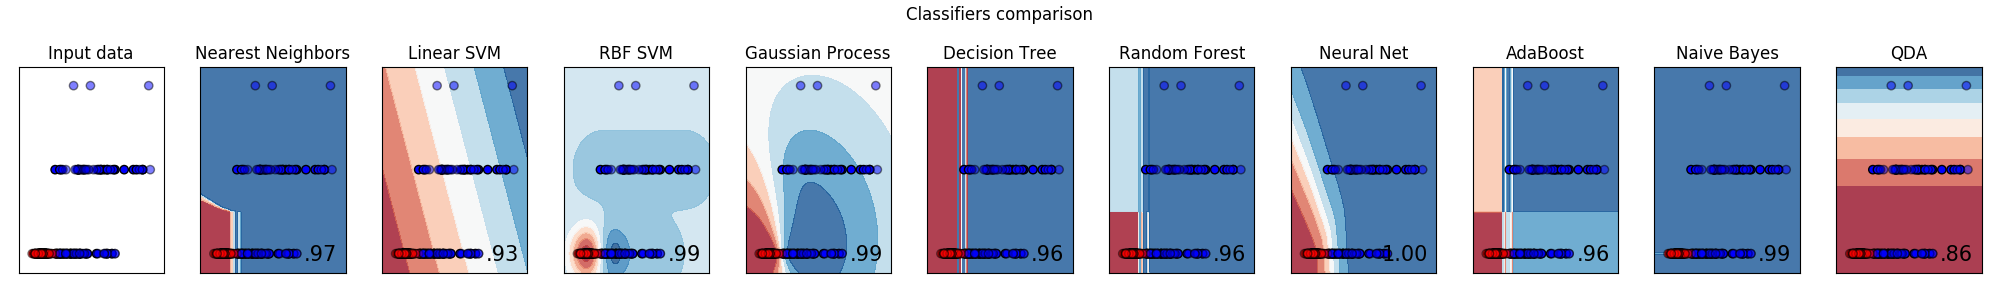
\includegraphics[width=2.5in]{classifiers-comparison-length-subdomains}
\caption{Example Figure}
\label{fig}
\end{figure}

\section{Including Citations}
Using BibTex it is easy to include citations to referenced works.
For example, we can cite the single work on OSI \cite{OSI} or a
number of works on common topic \cite{bellare04security,rfc2616,yi,SSL}.
We can also arrange for the list of references to appear at the end of
the paper.

\section{Conclusions}
Normally we finish a document with some conclusions.

\section*{Acknowledgements}

And we may even include some acknowledgements.

\bibliographystyle{abbrv}
\bibliography{paper}

\end{document}
